\section{Анализ требований к программному средству и разработка функциональных требований}
\label{sec:domain}

\subsection{Варианты использования программного средства}
\label{sec:domain:use_cases}

По результатам анализа предметной области и существующих аналогов можно сделать вывод, что проектируемое программное средство должно поддерживать ряд функций для автоматизации некоторых процессов учёта персонального бюджета, ключевыми из которых являются следующие:

\begin{itemize}
    \item \emph{Поддержка множественных валют}. Возможность учитывать расходы и доходы в различных приносит большую гибкость и повышает удобство пользования приложением.
    \item \emph{Управление счетами}, которое позволяет полностью манипулировать существующими источниками средств пользователя.
    \item \emph{Отображение списка счетов}, позволяющее наглядно видеть расположение и количество текущих денежных средств.
    \item \emph{Сводные значения по счетам}. Возможность общая сумма по всем валютам и количество денег, которые можно потратить до следующей зарплаты, являются крайне полезной информацией для контроля личных средств и избавления от лишних трат.
    \item \emph{Управление категориями} доходов и расходов, которые помогают распределить денежные траты для последующего анализа и оптимизации расходов.
    \item \emph{Просмотр статистики по категориям} позволит определить наиболее затратные категории расходов и узнать, куда конкретно уходят деньги.
    \item \emph{Управление транзакциями}. Функция является основной функцией проектируемого программного средства и позволяет регистрировать все операции с деньгами в системе.
    \item \emph{Отображение списка транзакций по дням} позволяет использовать просматривать и работать с существующими транзакциями.
\end{itemize}

Диаграмма вариантов использования, разработанная с использованием нотации \uml, представлена на рисунке~\ref{fig:domain:use_cases:model}.

\begin{figure}
    \centering
    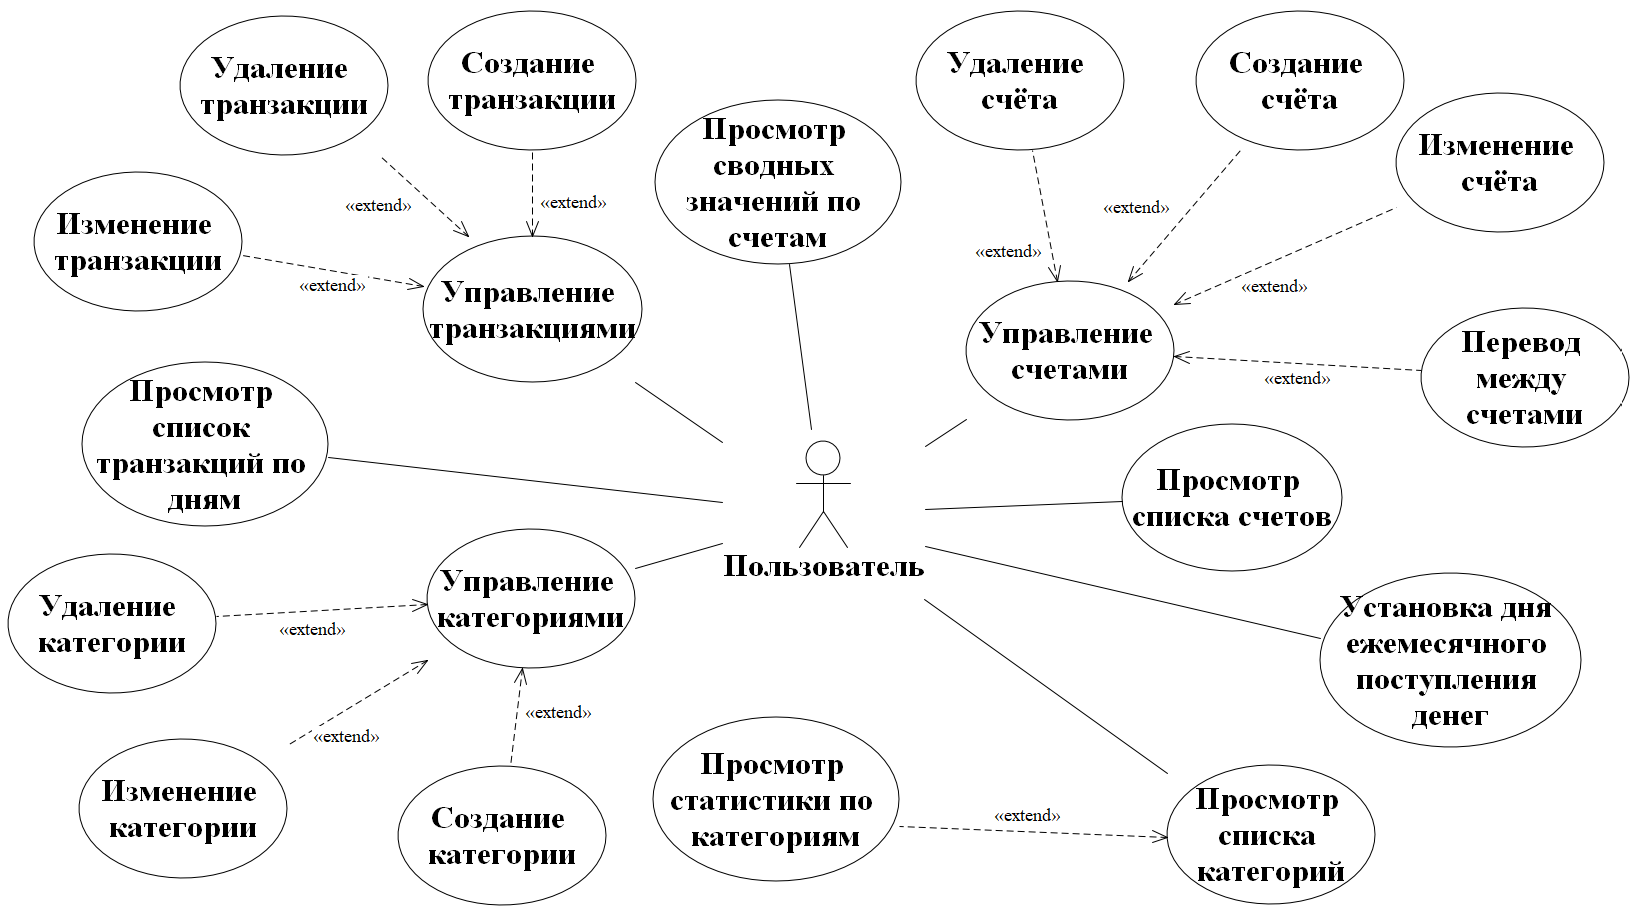
\includegraphics[scale=0.37]{2_1_use_case_model.png}
    \caption{Диаграмма вариантов использования ПС}
    \label{fig:domain:use_cases:model}
\end{figure}

Из диаграммы видно, что основные функции программного средства, а именно управление счетами, транзакциями и категориями, состоят из основных операций работы с данными, такими как создание, изменение и удаление соответствующего объекта.
Вместе с просмотром различных списков сущностей программного средства, данные варианты использования обеспечивают пользователю возможности по учёту доходов и расходов, описанные в подразделе~\ref{sec:analysis:literature:tracking}.

\emph{Просмотр статистики по категориям} позволяет пользователю оптимизировать расходы, обращая внимание на самые затратные категории расходов.

\emph{Сводные значения по счетам} могут быть использованы как основа для реализации любого из методов планирования бюджета, описанного в подразделе~\ref{sec:analysis:literature:planning}.

\subsection{Разработка инфологической модели базы данных}
\label{sec:domain:db}

Концептуальное (инфологическое) проектирование — построение семантической модели предметной области, то есть информационной модели наиболее высокого уровня абстракции.
Такая модель создаётся без ориентации на какую-либо конкретную СУБД и модель данных.
Основными конструктивными элементами инфологических моделей являются сущности, связи между ними и их свойства (атрибуты).

Исходя из необходимости использования в проектируемом приложении базы данных, разработаем ее инфологическую модель.
Для ее создания будем использовать расширение диаграммы классов \uml, предназначенное для моделирования баз данных.
Полученная диаграмма (рисунок~\ref{fig:domain:db:model}) будет являться моделью базы данных инфологического уровня~\cite{kulikov_db_workbook}.

\begin{figure}
    \centering
    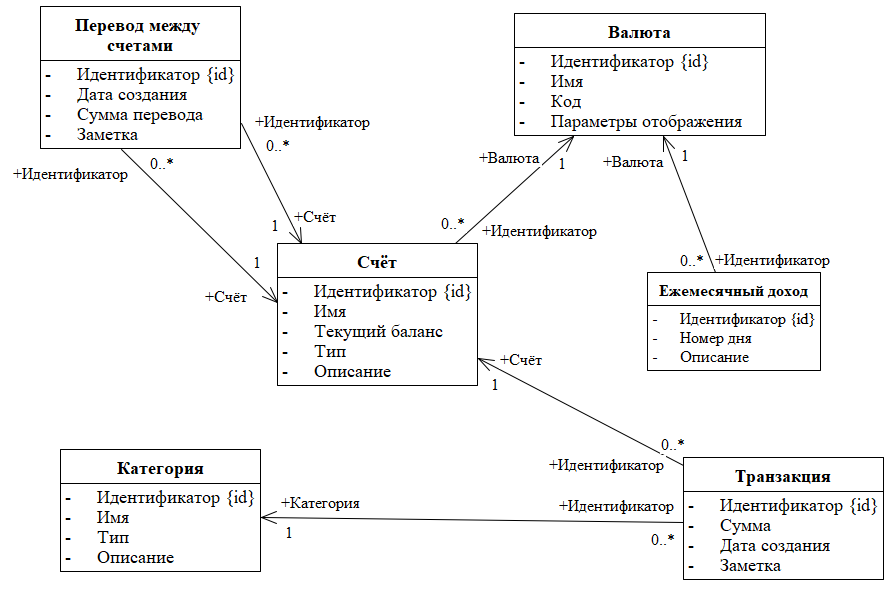
\includegraphics[scale=0.70]{2_2_logical_model.png}
    \caption{Инфологическая модель базы данных ПС}
    \label{fig:domain:db:model}
\end{figure}

Одной из особенностей разработанной модели является отсутствие сущности <<Пользователь>>.
Исходя из того, что под результатом дипломного проектирования предполагается \emph{однопользовательское} программное средство, разворачиваемое на мобильном устройстве -- ПС не нуждается в сохранении дополнительной информации о пользователе.
Однако, в будущем планируется ввести возможности по синхронизации данных с удаленным сервером.
При таком случае данные о пользователе, а именно данные аутентификации и авторизации, можно будет сохранить в локальном хранилище приложения.

Рассмотрим отдельно каждую из сущностей, представленной на диаграмме.

Сущность <<Валюта>> содержит информацию о денежных единицах, которая позволяет совершать пользователю работать с несколькими валютами одновременно.
Предполагается, что атрибут <<Код>> должен представляться в общепринятом трёхсимвольном коде валюты по стандарту ICO~4217~\cite{ico_4217}.
Атрибут <<Параметры отображения>> необходим для того, чтобы отображать конкретные денежные значения в общепринятом и знакомом для каждой валюты формате.

Сущность <<Счёт>> содержит актуальную информацию об пользовательском хранилище денежных средств.
<<Тип>> счета позволяет указать на то, является ли он сберегательным или нет.
Эта информация вносит больше гибкости в процесс планирования расходов и актуальна в момент расчета лимита расходов на день с учетом даты следующего поступления денег.
Данная сущность находится в связи с сущностью <<Валюта>>, так как каждый счёт хранит денежные средства той валюты, с которой связан.

Сущность <<Категория>> представляет собой отдельное направление расходов или доходов пользователя.
Атрибут <<Тип>> определяет вид транзакций, связанных с данной категорией и определяет, был совершен \emph{доход} или \emph{расход}.

Сущность <<Транзакция>> является основной в проектируемом программном средстве и определяет разовую операцию с денежными средствами.
Экземпляры сущности содержат в себе информацию о размере денежных средств, участвующих в операции, а также дату совершения операции.
<<Транзакция>> связана с сущностью <<Категория>>, благодаря чему можно определить, является ли конкретная транзакция расходом или доходом.
Также она связана с сущностью <<Счёт>>, что определяет валюту, в которой была проведена операция.

Сущность <<Денежный перевод>> содержит информацию о переносе денежных средств между двумя счетами проектируемого программного средства.
Данная сущность имеет две связи с сущностью <<Счёт>>, определяя, откуда и куда была перемещена сумма денег сумму денег.

Сущность <<Ежемесячный доход>> представляет данные о дате ожидаемого поступления денег и позволяет оценить количество денег, которые можно ежедневно тратить до такого поступления.
<<Ежемесячный доход>> связан с сущностью <<Валюта>>, так как расчёт лимита денег на день предполагается рассчитывать среди денег этой же валюты.

